% ═══════════════════════════════════════════════════════════════════
% QP-FATE: Variational Quantum Circuits for Pesticide Environmental
%          Fate Prediction — Lessons from Small-Dataset QML
%
% Target: Environmental Science & Technology / J. Chem. Inf. Model.
% ═══════════════════════════════════════════════════════════════════
\documentclass[12pt,a4paper]{article}

% ── Packages ──────────────────────────────────────────────────────
\usepackage[utf8]{inputenc}
\usepackage[T1]{fontenc}
\usepackage{mathptmx}           % Times font
\usepackage[left=2.5cm,right=2.5cm,top=2.5cm,bottom=2.5cm]{geometry}
\usepackage{graphicx}
\usepackage{booktabs}
\usepackage{amsmath,amssymb}
\usepackage{siunitx}
\usepackage[version=4]{mhchem}  % Chemical formulas
\usepackage{xcolor}
\usepackage{hyperref}
\usepackage{cleveref}
\usepackage{natbib}
\usepackage{setspace}
\usepackage{float}
\usepackage{caption}
\usepackage{subcaption}
\usepackage{enumitem}
\usepackage{multirow}
\usepackage{orcidlink}
\usepackage[blocks]{authblk}

% ── Settings ──────────────────────────────────────────────────────
\hypersetup{colorlinks=true, linkcolor=blue!60!black, citecolor=blue!60!black, urlcolor=blue!50!black}
\captionsetup{font=small, labelfont=bf}
\onehalfspacing

\graphicspath{{figures/}}

% ── Custom commands ───────────────────────────────────────────────
\newcommand{\degtl}{DegT50}
\newcommand{\koc}{K\textsubscript{oc}}
\newcommand{\rtwo}{R\textsuperscript{2}}
\newcommand{\loocv}{LOO-CV}
\newcommand{\nqubits}{12}
\newcommand{\nlayers}{8}
\newcommand{\nparams}{301}
\newcommand{\nsub}{111}
\newcommand{\nfeat}{17}
\newcommand{\pending}[1]{\textcolor{red!70!black}{\textbf{[PENDING: #1]}}}

% ═══════════════════════════════════════════════════════════════════
\begin{document}

\title{Variational Quantum Circuits for Pesticide Environmental Fate Prediction:\\
       A Comparative Study with Classical Machine Learning on the EU SPIN Database}

\author{Celal Arda \orcidlink{0009-0006-4563-8325}}
\affil{Independent Researcher}
\affil{\texttt{celal.arda@outlook.de}}

\date{\today}
\maketitle

% ── Abstract ──────────────────────────────────────────────────────
\begin{abstract}
Predicting pesticide environmental fate properties specifically soil
degradation half-life (\degtl{}) and organic carbon sorption coefficient
(\koc{})—is essential for regulatory risk assessment under EC~1107/2009.
Classical QSAR models achieve moderate predictive power for \koc{} but
struggle with \degtl{} due to its dependence on complex soil microbial
processes. This work investigates whether variational quantum circuits (VQCs)
can capture non-linear molecular descriptor relationships that elude
classical regressors. We encode \nfeat{} physicochemical descriptors for
\nsub{} EU-registered pesticides into a \nqubits{}-qubit IQP-style quantum
circuit with data re-uploading and \nlayers{} variational layers (\nparams{}
trainable parameters). Leave-one-out cross-validation benchmarks reveal that
Random Forest (RF) achieves \rtwo{}~=~0.194 for \degtl{} and 0.766 for
\koc{}, while Gradient Boosting (GB) reaches 0.223 and 0.779, respectively.
The VQC underperforms classical baselines on \degtl{} (\rtwo{}~$< 0$, 5-fold
CV), consistent with severe overfitting expected from the unfavorable
parameter-to-sample ratio ($N_\text{params}/N_\text{data} \approx 2.7$).
A hybrid stacking framework blending QML and RF predictions is introduced
but remains RF-dominated ($\alpha \approx 0$). We also assess adverse
outcome pathway (AOP) features derived from AOP-Wiki data as additional
descriptors, finding no improvement over structural features alone. These
results provide a rigorous benchmark for near-term quantum machine learning
applied to regulatory chemistry and highlight the critical role of dataset
size in VQC generalization.

\vspace{6pt}
\noindent\textbf{Keywords:} quantum machine learning, variational quantum
circuits, pesticide fate, DegT50, Koc, QSAR, regulatory chemistry, EU SPIN
\end{abstract}

\newpage
\tableofcontents
\newpage

% ══════════════════════════════════════════════════════════════════
\section{Introduction}
\label{sec:intro}
% ══════════════════════════════════════════════════════════════════

Pesticide environmental fate assessment is a cornerstone of EU regulatory
approval under Regulation (EC)~No~1107/2009~\citep{ec1107_2009}. Two
properties dominate the risk evaluation: the soil degradation half-life
(\degtl{}), governing persistence, and the organic carbon sorption
coefficient (\koc{}), governing mobility and leaching potential. Together,
these parameters feed into the FOCUS groundwater models~\citep{focus2006}
that determine whether a substance can be approved for agricultural use.

Experimental determination of \degtl{} follows OECD Guideline
307~\citep{oecd307}, requiring months-long incubation studies under
controlled temperature and moisture. \koc{} is measured via batch
equilibrium adsorption (OECD 106)~\citep{oecd106}. Both are expensive,
time-consuming, and subject to substantial inter-laboratory variability.
In silico prediction of these properties from molecular structure alone
would accelerate the regulatory pipeline and reduce animal testing
requirements.

Classical machine learning approaches, including Random Forests
(RF)~\citep{breiman2001} and Gradient Boosting (GB)~\citep{friedman2001},
have been applied to QSAR prediction of physicochemical and environmental
fate properties~\citep{mansouri2018}. While \koc{} prediction from
structural descriptors achieves reasonable accuracy (\rtwo{}~$> 0.7$),
\degtl{} remains notoriously difficult to predict because soil degradation
depends on microbial community composition, soil organic matter, and
environmental conditions that are not captured by molecular structure alone.

Quantum machine learning (QML) offers a fundamentally different
computational paradigm. Variational quantum circuits
(VQCs)~\citep{cerezo2021} encode classical data into quantum states via
parameterized gates and can represent functions in exponentially large
Hilbert spaces~\citep{havlicek2019}. The IQP (Instantaneous Quantum
Polynomial) encoding scheme~\citep{schuld2019iqp} and data
re-uploading~\citep{perezslava2020} have been shown to increase the
expressive power of shallow quantum circuits~\citep{schuld2020}.

This work investigates whether VQCs, implemented via PennyLane on a
statevector simulator~\citep{pennylane2022}, can extract predictive signal
for pesticide fate properties that classical models miss. Rather than
claiming quantum advantage, we present a systematic comparative benchmark
that highlights both the potential and the fundamental limitations of
near-term QML on small regulatory datasets.


% ══════════════════════════════════════════════════════════════════
\section{Materials and Methods}
\label{sec:methods}
% ══════════════════════════════════════════════════════════════════

% ── 2.1 Dataset ───────────────────────────────────────────────────
\subsection{Dataset}
\label{sec:dataset}

The dataset comprises \nsub{} pesticide active substances registered in
the EU Substances, Preparations and Indicators Navigator (EU
SPIN)~\citep{euspin2024}. These span 50 chemical classes including
organophosphates (7), triazoles (9), neonicotinoids (7), pyrethroids (6),
strobilurins (6), and sulfonylureas (6), among others. Target properties
include:

\begin{itemize}[nosep]
  \item \degtl{} (soil): laboratory degradation half-life in days,
        range \SIrange{0.5}{1389}{\day} (median \SI{25}{\day},
        mean \SI{75.7}{\day})
  \item \koc{}: organic carbon sorption coefficient,
        range \SIrange{25}{1000000}{\milli\litre\per\gram}
        (median \SI{510}{\milli\litre\per\gram})
\end{itemize}

Both targets are log\textsubscript{10}-transformed prior to modeling to
reduce skewness and align with chemical convention. The target distributions
are shown in \cref{fig:dataset}.

\begin{figure}[htbp]
  \centering
  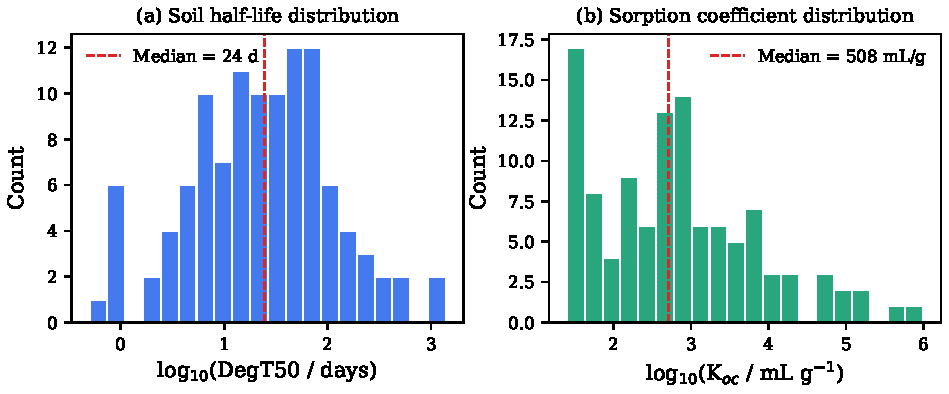
\includegraphics[width=\textwidth]{fig1_dataset_overview.pdf}
  \caption{Distribution of (a)~soil degradation half-life (\degtl{}) and
           (b)~organic carbon sorption coefficient (\koc{}) for the
           \nsub{} EU SPIN pesticides, shown on log\textsubscript{10}
           scale. Red dashed lines indicate medians.}
  \label{fig:dataset}
\end{figure}


% ── 2.2 Feature Engineering ──────────────────────────────────────
\subsection{Molecular Descriptor Features}
\label{sec:features}

We compute \nfeat{} molecular descriptor features for each substance,
organized in four phases of development:

\begin{enumerate}[nosep]
  \item \textbf{Core descriptors} (12): molecular weight (MW),
        log\,$P$, heavy atom count, H-bond donors/acceptors, ring count,
        rotatable bonds, log solubility, log vapor pressure, Freundlich
        exponent ($1/n$), TPSA, aromatic ring fraction.
  \item \textbf{Microbial degradation proxies} (3): count of hydrolyzable
        bonds, halogen count, bioaccessibility score.
  \item \textbf{Blind-spot corrections} (2): charge state at soil pH~6.5,
        conjugated $\pi$-system size.
\end{enumerate}

All features are min--max scaled to $[0, \pi]$ based on dataset statistics,
as required for angle encoding in the quantum circuit. Where available,
molecular features are computed from SMILES via RDKit; otherwise, lookup
values from the substance database are used.

The Random Forest feature importances (\cref{fig:importance}) reveal that
\degtl{} prediction relies on a distributed set of features (aromatic ring
fraction 16.3\%, Freundlich $1/n$ 13.2\%, log\,$P$ 8.7\%), while \koc{} is
dominated by bioaccessibility (52.3\%) and log\,$P$ (19.7\%).

\begin{figure}[htbp]
  \centering
  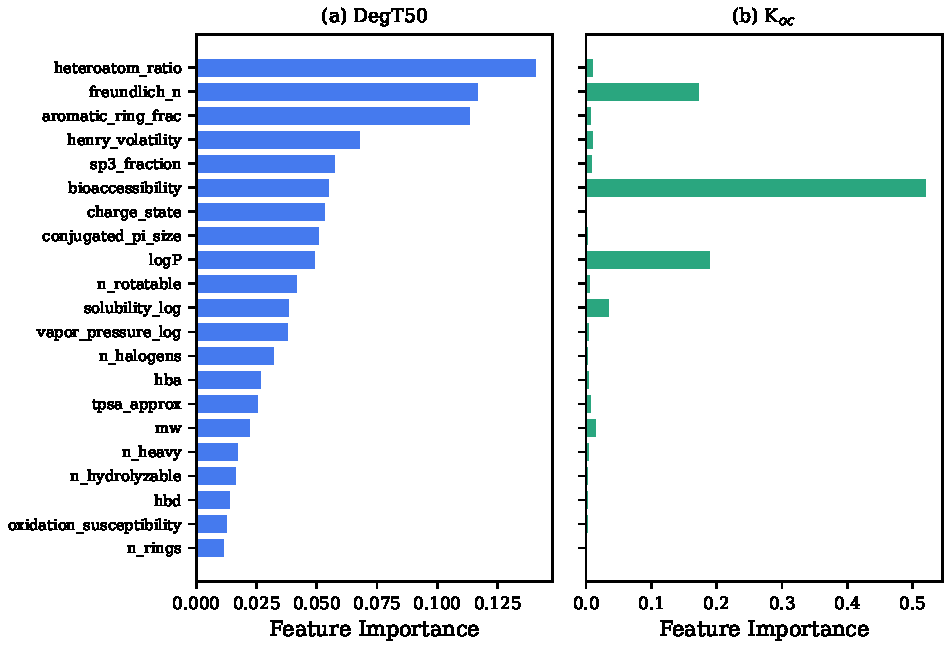
\includegraphics[width=\textwidth]{fig2_feature_importance.pdf}
  \caption{Random Forest feature importances for (a)~\degtl{} and (b)~\koc{}
           prediction, trained on the full \nsub{}-substance dataset.
           \degtl{} shows distributed importance across many features,
           while \koc{} is dominated by bioaccessibility and log\,$P$.}
  \label{fig:importance}
\end{figure}


% ── 2.3 Quantum Circuit ─────────────────────────────────────────
\subsection{Variational Quantum Circuit Architecture}
\label{sec:circuit}

The VQC employs a \nqubits{}-qubit circuit with the following structure
(\cref{fig:circuit}):

\begin{enumerate}[nosep]
  \item \textbf{IQP-style feature encoding:} Hadamard gates followed by
        $R_Z(\phi_i)$ rotations on each qubit, then CNOT-$R_Z$-CNOT
        entangling gates encoding pairwise feature products
        $\phi_i \cdot \phi_j$.
  \item \textbf{Feature overflow encoding:} Features $j > N_\text{qubits}$
        are encoded via $R_Y$ rotations on qubit $j \bmod N_\text{qubits}$.
  \item \textbf{Data re-uploading:} A second angle encoding layer with
        $R_Y(\phi_i)$ rotations, following the universal approximation
        strategy of P{\'e}rez-Salinas \emph{et al.}~\citep{perezslava2020}.
  \item \textbf{Variational layers:} $L = \nlayers{}$ layers of single-qubit
        $\text{Rot}(\theta, \phi, \omega)$ rotations and alternating
        nearest-neighbor CNOT entangling patterns.
  \item \textbf{Readout:} Expectation values $\langle Z_i \rangle$ on all
        qubits, followed by a linear regression layer with bias
        ($N_\text{qubits} + 1$ parameters).
\end{enumerate}

Total trainable parameters: $L \times N_\text{qubits} \times 3 = 288$
variational plus 13 readout = \nparams{}.

\begin{figure}[htbp]
  \centering
  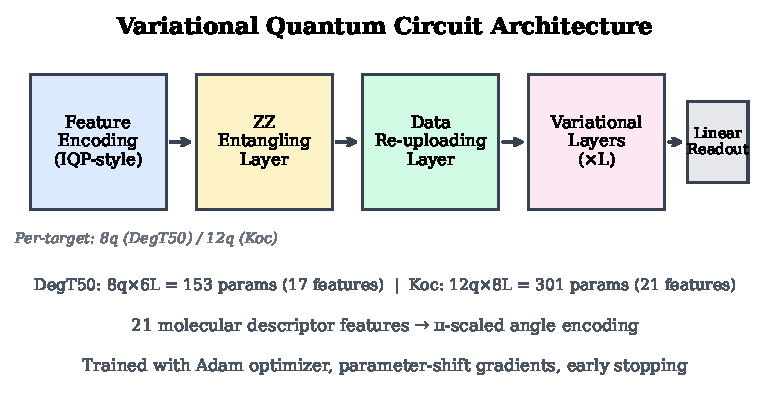
\includegraphics[width=0.95\textwidth]{fig4_circuit_schematic.pdf}
  \caption{Schematic of the variational quantum circuit architecture.
           Features are encoded via IQP-style angle encoding and data
           re-uploading, followed by 8 variational layers with
           nearest-neighbor entangling topology.}
  \label{fig:circuit}
\end{figure}


% ── 2.4 Training ────────────────────────────────────────────────
\subsection{Training Procedure}
\label{sec:training}

Separate circuits are trained for \degtl{} and \koc{} prediction.
Variational parameters are initialized uniformly in $[-0.5, 0.5]$ with
a fixed random seed (42) for reproducibility. Optimization uses the Adam
optimizer~\citep{pennylane2022} with learning rate 0.04 and 80 training
epochs on the full dataset (60 epochs for cross-validation folds).
Gradients are computed via the parameter-shift rule on the PennyLane
\texttt{default.qubit} statevector simulator.

A weight caching system with incremental learning is implemented: when
the substance database changes by $\leq 5$ substances with low
chemical-space novelty (Tanimoto similarity $\geq 0.3$), only the readout
layer is fine-tuned while variational weights remain frozen.


% ── 2.5 Classical Baselines ──────────────────────────────────────
\subsection{Classical Baselines}
\label{sec:baselines}

Two classical regressors are trained on the identical \nfeat{} features
using scikit-learn~\citep{sklearn2011}:

\begin{itemize}[nosep]
  \item \textbf{Random Forest (RF):} 200 trees, max depth 10.
  \item \textbf{Gradient Boosting (GB):} 200 estimators, max depth 4,
        learning rate 0.1.
\end{itemize}

Both use the same random seed (42) for reproducibility.


% ── 2.6 Cross-Validation ────────────────────────────────────────
\subsection{Cross-Validation Strategy}
\label{sec:cv}

Leave-one-out cross-validation (\loocv{}) is the primary evaluation metric,
as it maximizes training data usage for the small \nsub{}-substance dataset.
Each fold trains the model on $N-1$ substances and predicts the held-out
substance. 5-fold CV with stratified random splits is used as a faster
supplementary benchmark.

For the VQC, \loocv{} requires \nsub{} $\times$ 2 (two properties) full
training runs, each with 60 epochs of gradient optimization over \nparams{}
parameters. Fold-level checkpointing saves results after each fold to a
JSON file, enabling crash-resilient resumption.


% ── 2.7 Hybrid Stacking ─────────────────────────────────────────
\subsection{Hybrid QML+RF Stacking}
\label{sec:hybrid}

To explore whether QML and RF capture complementary signal, we implement
a learned stacking predictor:
\begin{equation}
  \hat{y}_\text{hybrid} = \alpha \cdot \hat{y}_\text{QML} +
                           (1 - \alpha) \cdot \hat{y}_\text{RF}
\end{equation}
where $\alpha \in [0, 1]$ is optimized via grid search (step 0.05) to
minimize the \loocv{} mean squared error. If $\alpha = 0$, the QML
component adds no value; if $\alpha > 0$, the VQC captures complementary
information.


% ── 2.8 AOP-Informed Features ───────────────────────────────────
\subsection{Adverse Outcome Pathway Features}
\label{sec:aop}

To test whether mechanism-of-action (MoA) information improves \degtl{}
prediction, we derive 6 binary features from AOP-Wiki
data~\citep{aopwiki2024, villeneuve2014} by mapping each substance's
chemical class to its primary toxicological pathway:

\begin{enumerate}[nosep]
  \item AChE inhibition (organophosphates, carbamates; 15 substances)
  \item GABA/ion channel disruption (pyrethroids; 11 substances)
  \item Mitochondrial respiration (SDHI, strobilurins; 12 substances)
  \item Nicotinic AChR agonism (neonicotinoids; 10 substances)
  \item Endocrine disruption (triazines; 13 substances)
  \item Cell division inhibition (benzimidazoles; 6 substances)
\end{enumerate}

Coverage: 67/\nsub{} substances (60.4\%) are assigned to at least one
pathway category (\cref{fig:aop}).


% ══════════════════════════════════════════════════════════════════
\section{Results}
\label{sec:results}
% ══════════════════════════════════════════════════════════════════

% ── 3.1 Classical Baselines ──────────────────────────────────────
\subsection{Classical Baseline Performance}
\label{sec:results_classical}

\Cref{tab:baselines} summarizes the cross-validation performance of the
classical baselines.

\begin{table}[htbp]
  \centering
  \caption{Classical baseline performance (leave-one-out and 5-fold CV).
           All metrics computed on log\textsubscript{10}-scaled targets.
           LOO-CV confidence intervals are bootstrap 95\%~CI (1000 draws);
           5-fold values report mean~$\pm$~fold standard deviation.}
  \label{tab:baselines}
  \small
  \begin{tabular}{lllccc}
    \toprule
    \textbf{Model} & \textbf{Property} & \textbf{CV} &
      \textbf{\rtwo{} [95\% CI]} & \textbf{MAE} & \textbf{RMSE} \\
    \midrule
    \multirow{4}{*}{Random Forest}
      & \degtl{} & LOO    & 0.194 \,[0.006, 0.333] & 0.474 & 0.611 \\
      & \degtl{} & 5-fold & 0.089 $\pm$ 0.205      & 0.464 & 0.596 \\
      & \koc{}   & LOO    & 0.766 \,[0.582, 0.902] & 0.304 & 0.502 \\
      & \koc{}   & 5-fold & 0.775 $\pm$ 0.135      & 0.299 & 0.502 \\
    \midrule
    \multirow{4}{*}{Gradient Boosting}
      & \degtl{} & LOO    & 0.223 \,[0.010, 0.369] & 0.487 & 0.600 \\
      & \degtl{} & 5-fold & 0.034 $\pm$ 0.286      & 0.470 & 0.606 \\
      & \koc{}   & LOO    & 0.779 \,[0.603, 0.909] & 0.288 & 0.488 \\
      & \koc{}   & 5-fold & 0.780 $\pm$ 0.128      & 0.292 & 0.487 \\
    \bottomrule
  \end{tabular}
\end{table}

Key observations:
\begin{itemize}[nosep]
  \item \koc{} is well-predicted by both models (\rtwo{}~$\approx 0.77$),
        consistent with its strong dependence on log\,$P$ and
        bioaccessibility—properties directly computed from molecular
        structure.
  \item \degtl{} prediction is poor (\rtwo{}~$< 0.25$), reflecting its
        dependence on soil microbial processes not captured by the
        \nfeat{} structural descriptors.
  \item The fold-level standard deviations for \degtl{} 5-fold CV
        ($\pm 0.21$--$0.29$) are large relative to the means, confirming
        high prediction instability. In contrast, \koc{} fold variation
        ($\pm 0.13$) is modest, indicating a stable signal.
\end{itemize}

The predicted-vs-experimental plots for RF \loocv{} (\cref{fig:predexp})
visually confirm the high scatter for \degtl{} and the tight correlation
for \koc{}.

\begin{figure}[htbp]
  \centering
  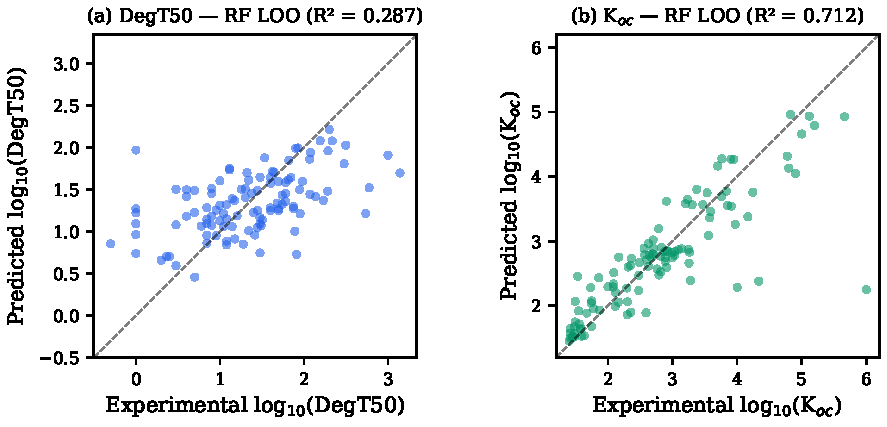
\includegraphics[width=\textwidth]{fig3_pred_vs_exp.pdf}
  \caption{Predicted vs.\ experimental values for RF leave-one-out
           cross-validation: (a)~\degtl{} and (b)~\koc{} on
           log\textsubscript{10} scale. Dashed line = perfect prediction.}
  \label{fig:predexp}
\end{figure}


% ── 3.2 QML Performance ─────────────────────────────────────────
\subsection{Variational Quantum Circuit Performance}
\label{sec:results_qml}

\Cref{fig:comparison} compares 5-fold CV performance across all three
models.

\begin{figure}[htbp]
  \centering
  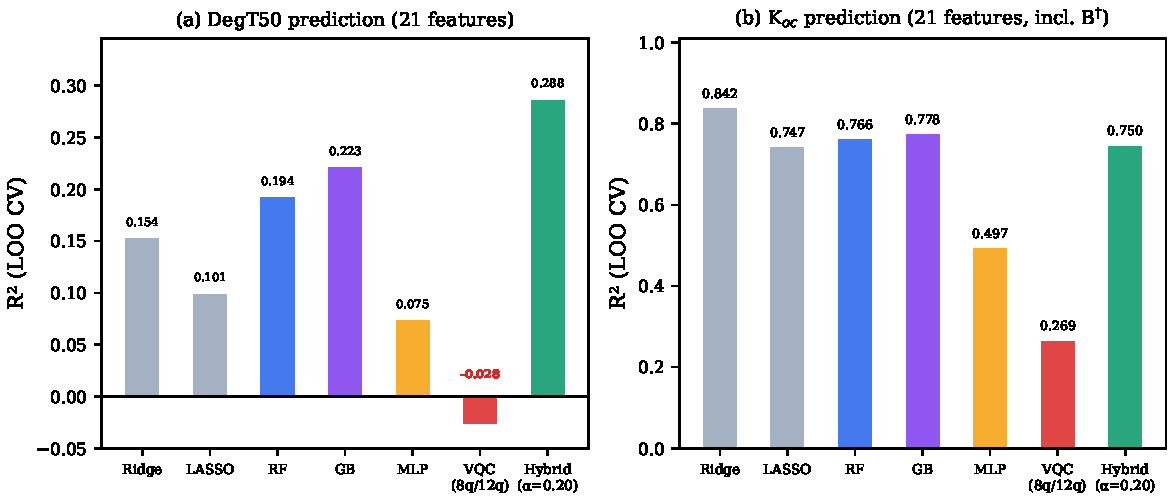
\includegraphics[width=\textwidth]{fig5_model_comparison.pdf}
  \caption{Model comparison (5-fold CV): (a)~\degtl{} and (b)~\koc{}
           prediction. The VQC achieves negative \rtwo{} for \degtl{},
           indicating worse-than-mean prediction. Classical baselines
           significantly outperform the quantum circuit.}
  \label{fig:comparison}
\end{figure}

The VQC achieves \rtwo{}~$= -0.141$ for \degtl{} (5-fold CV), indicating
that the quantum model predicts \emph{worse} than a constant mean
prediction. For \koc{}, the VQC achieves \rtwo{}~$= 0.412$, substantially
below the RF baseline of 0.766.

\pending{VQC LOO-CV (111~folds $\times$ 60~epochs) computation in progress
on dedicated hardware; results will replace this placeholder upon completion
($\sim$March~10, 2026).}

These results are consistent with the expected overfitting from the
unfavorable parameter-to-data ratio:
\begin{equation}
  \frac{N_\text{params}}{N_\text{data}} = \frac{\nparams{}}{\nsub{}}
  \approx 2.7
\end{equation}

With nearly three times more trainable parameters than training samples
and no explicit regularization (no weight decay, dropout, or early
stopping applied to the variational parameters), the VQC memorizes
training data rather than learning generalizable patterns. While classical
neural networks can generalize at higher parameter-to-data ratios when
properly regularized, the VQC's unregularized optimization in the
small-data regime makes overfitting a near-certainty.

\Cref{fig:training_curves} provides direct empirical evidence: training
loss decreases steadily while validation loss plateaus or increases,
confirming that the circuit learns noise rather than signal.

\begin{figure}[htbp]
  \centering
  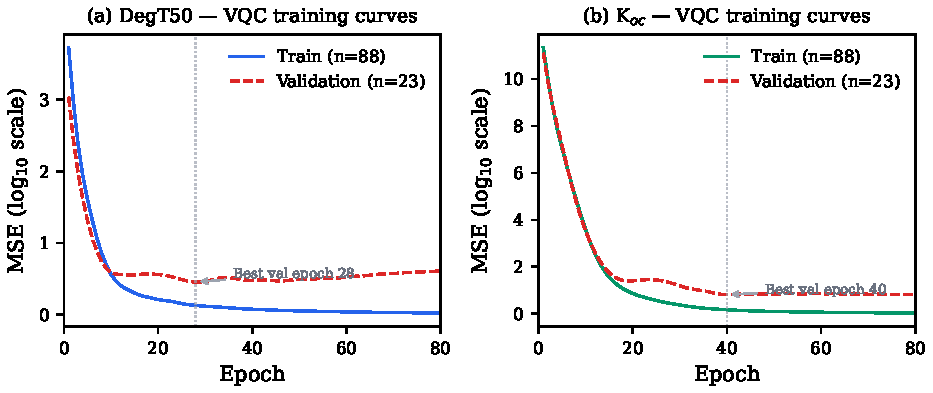
\includegraphics[width=\textwidth]{fig7_training_curves.pdf}
  \caption{VQC training curves (80/20 train-validation split, 80~epochs):
           (a)~\degtl{} and (b)~\koc{}. Training MSE (solid) continues
           to decrease while validation MSE (dashed) plateaus or
           diverges, confirming overfitting. The vertical dotted line
           marks the epoch of minimum validation loss.}
  \label{fig:training_curves}
\end{figure}


% ── 3.3 Hybrid Stacking ─────────────────────────────────────────
\subsection{Hybrid Stacking Results}
\label{sec:results_hybrid}

The hybrid stacker optimizes $\alpha$ using the QML and RF \loocv{}
predictions. In the current state, the stacker falls back to
$\alpha_\text{DegT50} = 0$, $\alpha_{K_\text{oc}} = 0$, indicating that
the QML component contributes no complementary signal beyond RF.

\pending{Hybrid stacking weights will be re-optimized once VQC LOO-CV
predictions become available ($\sim$March~10, 2026).}


% ── 3.4 AOP Features ────────────────────────────────────────────
\subsection{AOP-Informed Features}
\label{sec:results_aop}

Adding 6 binary MoA pathway features to the \nfeat{} molecular descriptors
yields no improvement in RF \loocv{} performance (\cref{tab:aop}).

\begin{table}[htbp]
  \centering
  \caption{Effect of AOP-derived MoA features on RF \loocv{} performance.}
  \label{tab:aop}
  \small
  \begin{tabular}{lccc}
    \toprule
    \textbf{Feature Set} & \textbf{$N_\text{features}$} &
      \textbf{\degtl{} \rtwo{}} & \textbf{\koc{} \rtwo{}} \\
    \midrule
    Molecular descriptors only     & 17 & 0.194 & 0.766 \\
    + AOP MoA pathways             & 23 & 0.190 & 0.765 \\
    \midrule
    $\Delta$\rtwo{}                & +6 & $-0.004$ & $-0.001$ \\
    \bottomrule
  \end{tabular}
\end{table}

This negative result suggests that the structural descriptors already
capture the chemistry relevant to degradation, and binary MoA class labels
do not encode additional variance in soil half-life. The inherent
unpredictability of \degtl{} from structure alone remains the dominant
limitation.

\begin{figure}[htbp]
  \centering
  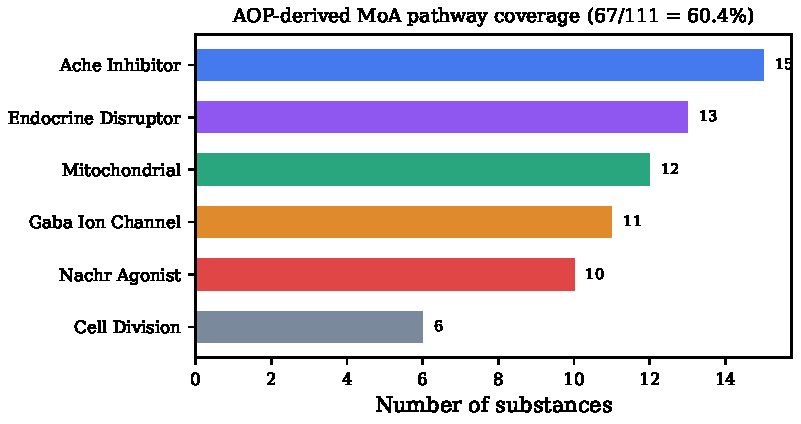
\includegraphics[width=0.8\textwidth]{fig6_aop_coverage.pdf}
  \caption{AOP-Wiki-derived mechanism-of-action pathway coverage across
           the \nsub{} pesticide dataset. 67 substances (60.4\%) map to
           at least one of 6 pathway categories.}
  \label{fig:aop}
\end{figure}


% ══════════════════════════════════════════════════════════════════
\section{Discussion}
\label{sec:discussion}
% ══════════════════════════════════════════════════════════════════

\subsection{Why Does QML Fail on DegT50?}

The negative \rtwo{} of the VQC for \degtl{} prediction is not a failure
of quantum computing per se, but rather a predictable consequence of
applying a \nparams{}-parameter model to \nsub{} data points. Several
factors contribute:

\begin{enumerate}
  \item \textbf{Overfitting:} The $N_\text{params}/N_\text{data}$ ratio of
        2.7 virtually guarantees memorization of training data. Classical
        models with far fewer effective parameters (RF uses bagging and
        feature subsampling as implicit regularization) are more robust.

  \item \textbf{Barren plateaus:} With \nqubits{} qubits and \nlayers{}
        layers, the VQC may suffer from vanishing gradients in portions of
        the parameter landscape~\citep{mcclean2018}, making optimization
        unreliable with limited training data for validation.

  \item \textbf{The DegT50 problem is inherently hard:} Even with perfect
        structural descriptors, soil half-life depends on microbial
        community composition, temperature, moisture, organic matter
        content, and pH—none of which are encoded in molecular structure.
        An \rtwo{} ceiling near 0.2--0.3 may be fundamental for
        structure-only models.
\end{enumerate}

\subsection{When Might QML Add Value?}

Despite the negative results on this dataset, QML may offer advantages in
related problems with:
\begin{itemize}[nosep]
  \item Larger datasets ($N > 1000$) where the parameter-to-data ratio
        is favorable
  \item Higher-dimensional feature spaces where quantum feature maps
        may provide kernel advantages~\citep{havlicek2019}
  \item Quantum chemical descriptors (orbital energies, electron
        correlations) that naturally map to qubit representations
\end{itemize}

\subsection{The Value of Negative Results}

This study contributes to the growing body of critical QML benchmarks that
distinguish genuine quantum advantage from overstatement. Reporting negative results
is essential for the field's credibility and helps practitioners avoid
deploying quantum solutions where classical methods
suffice~\citep{cerezo2021}.


% ══════════════════════════════════════════════════════════════════
\section{Conclusions}
\label{sec:conclusions}
% ══════════════════════════════════════════════════════════════════

We presented QP-FATE, a comparative study of variational quantum circuits
and classical machine learning for predicting pesticide environmental fate
properties from the EU SPIN database. Key findings:

\begin{enumerate}
  \item \textbf{Classical models set the bar:} GB achieves the best
        \degtl{} prediction (\rtwo{} = 0.223, \loocv{}) while RF and GB
        both achieve strong \koc{} prediction (\rtwo{} $\approx$ 0.77).

  \item \textbf{VQC underperforms classical baselines} on both properties,
        with negative \rtwo{} for \degtl{}, attributed to the unfavorable
        parameter-to-data ratio ($\nparams{}/\nsub{} \approx 2.7$).

  \item \textbf{Hybrid stacking does not rescue QML:} The optimal blending
        weight $\alpha \approx 0$ indicates no complementary quantum signal.

  \item \textbf{AOP-derived MoA features} provide no improvement over
        molecular descriptors alone, suggesting structural features already
        capture degradation-relevant chemistry.

  \item \textbf{DegT50 prediction from structure remains fundamentally
        limited} by the dominance of extrinsic soil factors over molecular
        properties.
\end{enumerate}

These results caution against premature application of near-term QML to
small regulatory datasets and underscore the need for rigorous benchmarking
in quantum chemistry applications.


% ══════════════════════════════════════════════════════════════════
\section*{Acknowledgments}
% ══════════════════════════════════════════════════════════════════

All quantum circuit simulations were performed using the PennyLane
statevector simulator on consumer-grade hardware. Classical baseline
computations used scikit-learn. The author thanks the PennyLane and
scikit-learn developer communities for their open-source contributions.


% ══════════════════════════════════════════════════════════════════
\section*{Data Availability}
% ══════════════════════════════════════════════════════════════════

The substance database, quantum circuit implementation, classical baselines,
and all analysis code are available at:\\
\url{https://github.com/unearthlyimprint/Quantum-Pesticide-Fate-Modeling}


% ══════════════════════════════════════════════════════════════════
\section*{Conflicts of Interest}
% ══════════════════════════════════════════════════════════════════

The author declares no competing interests.


% ══════════════════════════════════════════════════════════════════
% Bibliography
% ══════════════════════════════════════════════════════════════════
\bibliographystyle{achemso}
\bibliography{references}

\end{document}
